\documentclass[1p]{elsarticle_modified}
%\bibliographystyle{elsarticle-num}

%\usepackage[colorlinks]{hyperref}
%\usepackage{abbrmath_seonhwa} %\Abb, \Ascr, \Acal ,\Abf, \Afrak
\usepackage{amsfonts}
\usepackage{amssymb}
\usepackage{amsmath}
\usepackage{amsthm}
\usepackage{scalefnt}
\usepackage{amsbsy}
\usepackage{kotex}
\usepackage{caption}
\usepackage{subfig}
\usepackage{color}
\usepackage{graphicx}
\usepackage{xcolor} %% white, black, red, green, blue, cyan, magenta, yellow
\usepackage{float}
\usepackage{setspace}
\usepackage{hyperref}

\usepackage{tikz}
\usetikzlibrary{arrows}

\usepackage{multirow}
\usepackage{array} % fixed length table
\usepackage{hhline}

%%%%%%%%%%%%%%%%%%%%%
\makeatletter
\renewcommand*\env@matrix[1][\arraystretch]{%
	\edef\arraystretch{#1}%
	\hskip -\arraycolsep
	\let\@ifnextchar\new@ifnextchar
	\array{*\c@MaxMatrixCols c}}
\makeatother %https://tex.stackexchange.com/questions/14071/how-can-i-increase-the-line-spacing-in-a-matrix
%%%%%%%%%%%%%%%

\usepackage[normalem]{ulem}

\newcommand{\msout}[1]{\ifmmode\text{\sout{\ensuremath{#1}}}\else\sout{#1}\fi}
%SOURCE: \msout is \stkout macro in https://tex.stackexchange.com/questions/20609/strikeout-in-math-mode

\newcommand{\cancel}[1]{
	\ifmmode
	{\color{red}\msout{#1}}
	\else
	{\color{red}\sout{#1}}
	\fi
}

\newcommand{\add}[1]{
	{\color{blue}\uwave{#1}}
}

\newcommand{\replace}[2]{
	\ifmmode
	{\color{red}\msout{#1}}{\color{blue}\uwave{#2}}
	\else
	{\color{red}\sout{#1}}{\color{blue}\uwave{#2}}
	\fi
}

\newcommand{\Sol}{\mathcal{S}} %segment
\newcommand{\D}{D} %diagram
\newcommand{\A}{\mathcal{A}} %arc


%%%%%%%%%%%%%%%%%%%%%%%%%%%%%5 test

\def\sl{\operatorname{\textup{SL}}(2,\Cbb)}
\def\psl{\operatorname{\textup{PSL}}(2,\Cbb)}
\def\quan{\mkern 1mu \triangleright \mkern 1mu}

\theoremstyle{definition}
\newtheorem{thm}{Theorem}[section]
\newtheorem{prop}[thm]{Proposition}
\newtheorem{lem}[thm]{Lemma}
\newtheorem{ques}[thm]{Question}
\newtheorem{cor}[thm]{Corollary}
\newtheorem{defn}[thm]{Definition}
\newtheorem{exam}[thm]{Example}
\newtheorem{rmk}[thm]{Remark}
\newtheorem{alg}[thm]{Algorithm}

\newcommand{\I}{\sqrt{-1}}
\begin{document}

%\begin{frontmatter}
%
%\title{Boundary parabolic representations of knots up to 8 crossings}
%
%%% Group authors per affiliation:
%\author{Yunhi Cho} 
%\address{Department of Mathematics, University of Seoul, Seoul, Korea}
%\ead{yhcho@uos.ac.kr}
%
%
%\author{Seonhwa Kim} %\fnref{s_kim}}
%\address{Center for Geometry and Physics, Institute for Basic Science, Pohang, 37673, Korea}
%\ead{ryeona17@ibs.re.kr}
%
%\author{Hyuk Kim}
%\address{Department of Mathematical Sciences, Seoul National University, Seoul 08826, Korea}
%\ead{hyukkim@snu.ac.kr}
%
%\author{Seokbeom Yoon}
%\address{Department of Mathematical Sciences, Seoul National University, Seoul, 08826,  Korea}
%\ead{sbyoon15@snu.ac.kr}
%
%\begin{abstract}
%We find all boundary parabolic representation of knots up to 8 crossings.
%
%\end{abstract}
%\begin{keyword}
%    \MSC[2010] 57M25 
%\end{keyword}
%
%\end{frontmatter}

%\linenumbers
%\tableofcontents
%
\newcommand\colored[1]{\textcolor{white}{\rule[-0.35ex]{0.8em}{1.4ex}}\kern-0.8em\color{red} #1}%
%\newcommand\colored[1]{\textcolor{white}{ #1}\kern-2.17ex	\textcolor{white}{ #1}\kern-1.81ex	\textcolor{white}{ #1}\kern-2.15ex\color{red}#1	}

{\Large $\underline{11a_{313}~(K11a_{313})}$}

\setlength{\tabcolsep}{10pt}
\renewcommand{\arraystretch}{1.6}
\vspace{1cm}\begin{tabular}{m{100pt}>{\centering\arraybackslash}m{274pt}}
\multirow{5}{120pt}{
	\centering
	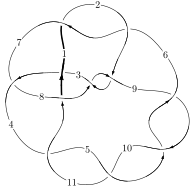
\includegraphics[width=112pt]{../../../GIT/diagram.site/Diagrams/png/562_11a_313.png}\\
\ \ \ A knot diagram\footnotemark}&
\allowdisplaybreaks
\textbf{Linearized knot diagam} \\
\cline{2-2}
 &
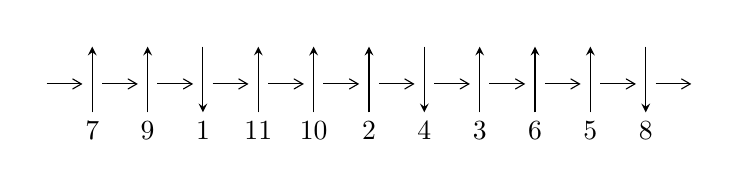
\begin{tikzpicture}[x=20pt, y=17pt]
	% nodes
	\node (C0) at (0, 0) {};
	\node (C1) at (1, 0) {};
	\node (C1U) at (1, +1) {};
	\node (C1D) at (1, -1) {7};

	\node (C2) at (2, 0) {};
	\node (C2U) at (2, +1) {};
	\node (C2D) at (2, -1) {9};

	\node (C3) at (3, 0) {};
	\node (C3U) at (3, +1) {};
	\node (C3D) at (3, -1) {1};

	\node (C4) at (4, 0) {};
	\node (C4U) at (4, +1) {};
	\node (C4D) at (4, -1) {11};

	\node (C5) at (5, 0) {};
	\node (C5U) at (5, +1) {};
	\node (C5D) at (5, -1) {10};

	\node (C6) at (6, 0) {};
	\node (C6U) at (6, +1) {};
	\node (C6D) at (6, -1) {2};

	\node (C7) at (7, 0) {};
	\node (C7U) at (7, +1) {};
	\node (C7D) at (7, -1) {4};

	\node (C8) at (8, 0) {};
	\node (C8U) at (8, +1) {};
	\node (C8D) at (8, -1) {3};

	\node (C9) at (9, 0) {};
	\node (C9U) at (9, +1) {};
	\node (C9D) at (9, -1) {6};

	\node (C10) at (10, 0) {};
	\node (C10U) at (10, +1) {};
	\node (C10D) at (10, -1) {5};

	\node (C11) at (11, 0) {};
	\node (C11U) at (11, +1) {};
	\node (C11D) at (11, -1) {8};
	\node (C12) at (12, 0) {};

	% arrows
	\draw[->,>={angle 60}]
	(C0) edge (C1) (C1) edge (C2) (C2) edge (C3) (C3) edge (C4) (C4) edge (C5) (C5) edge (C6) (C6) edge (C7) (C7) edge (C8) (C8) edge (C9) (C9) edge (C10) (C10) edge (C11) (C11) edge (C12) ;	\draw[->,>=stealth]
	(C1D) edge (C1U) (C2D) edge (C2U) (C3U) edge (C3D) (C4D) edge (C4U) (C5D) edge (C5U) (C6D) edge (C6U) (C7U) edge (C7D) (C8D) edge (C8U) (C9D) edge (C9U) (C10D) edge (C10U) (C11U) edge (C11D) ;
	\end{tikzpicture} \\
\hhline{~~} \\& 
\textbf{Solving Sequence} \\ \cline{2-2} 
 &
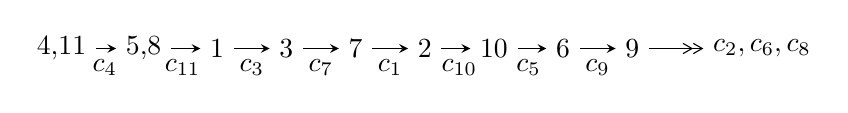
\begin{tikzpicture}[x=25pt, y=7pt]
	% node
	\node (A0) at (-1/8, 0) {4,11};
	\node (A1) at (17/16, 0) {5,8};
	\node (A2) at (17/8, 0) {1};
	\node (A3) at (25/8, 0) {3};
	\node (A4) at (33/8, 0) {7};
	\node (A5) at (41/8, 0) {2};
	\node (A6) at (49/8, 0) {10};
	\node (A7) at (57/8, 0) {6};
	\node (A8) at (65/8, 0) {9};
	\node (C1) at (1/2, -1) {$c_{4}$};
	\node (C2) at (13/8, -1) {$c_{11}$};
	\node (C3) at (21/8, -1) {$c_{3}$};
	\node (C4) at (29/8, -1) {$c_{7}$};
	\node (C5) at (37/8, -1) {$c_{1}$};
	\node (C6) at (45/8, -1) {$c_{10}$};
	\node (C7) at (53/8, -1) {$c_{5}$};
	\node (C8) at (61/8, -1) {$c_{9}$};
	\node (A9) at (10, 0) {$c_{2},c_{6},c_{8}$};

	% edge
	\draw[->,>=stealth]	
	(A0) edge (A1) (A1) edge (A2) (A2) edge (A3) (A3) edge (A4) (A4) edge (A5) (A5) edge (A6) (A6) edge (A7) (A7) edge (A8) ;
	\draw[->>,>={angle 60}]	
	(A8) edge (A9);
\end{tikzpicture} \\ 

\end{tabular} \\

\footnotetext{
The image of knot diagram is generated by the software ``\textbf{Draw programme}" developed by Andrew Bartholomew(\url{http://www.layer8.co.uk/maths/draw/index.htm\#Running-draw}), where we modified some parts for our purpose(\url{https://github.com/CATsTAILs/LinksPainter}).
}\phantom \\ \newline 
\centering \textbf{Ideals for irreducible components\footnotemark of $X_{\text{par}}$} 
 
\begin{align*}
I^u_{1}&=\langle 
-5 u^{17}-33 u^{16}+\cdots+4 b-52,\;13 u^{17}+81 u^{16}+\cdots+8 a+96,\;u^{18}+7 u^{17}+\cdots+76 u+8\rangle \\
I^u_{2}&=\langle 
-2 a^5 u^4+3 a^4 u^4+\cdots+4 a+1,\;-3 a^5 u^4+2 a^4 u^4+\cdots-19 a+171,\;u^5- u^4+4 u^3-3 u^2+3 u-1\rangle \\
I^u_{3}&=\langle 
- u^9-6 u^7-12 u^5-9 u^3- u^2+b-2 u-1,\;u^9- u^8+7 u^7-6 u^6+17 u^5-12 u^4+17 u^3-8 u^2+a+6 u,\\
\phantom{I^u_{3}}&\phantom{= \langle  }u^{10}+7 u^8+17 u^6+17 u^4+u^3+7 u^2+2 u+1\rangle \\
\\
\end{align*}
\raggedright * 3 irreducible components of $\dim_{\mathbb{C}}=0$, with total 58 representations.\\
\footnotetext{All coefficients of polynomials are rational numbers. But the coefficients are sometimes approximated in decimal forms when there is not enough margin.}
\newpage
\renewcommand{\arraystretch}{1}
\centering \section*{I. $I^u_{1}= \langle -5 u^{17}-33 u^{16}+\cdots+4 b-52,\;13 u^{17}+81 u^{16}+\cdots+8 a+96,\;u^{18}+7 u^{17}+\cdots+76 u+8 \rangle$}
\flushleft \textbf{(i) Arc colorings}\\
\begin{tabular}{m{7pt} m{180pt} m{7pt} m{180pt} }
\flushright $a_{4}=$&$\begin{pmatrix}1\\0\end{pmatrix}$ \\
\flushright $a_{11}=$&$\begin{pmatrix}0\\u\end{pmatrix}$ \\
\flushright $a_{5}=$&$\begin{pmatrix}1\\- u^2\end{pmatrix}$ \\
\flushright $a_{8}=$&$\begin{pmatrix}-\frac{13}{8} u^{17}-\frac{81}{8} u^{16}+\cdots-\frac{427}{4} u-12\\\frac{5}{4} u^{17}+\frac{33}{4} u^{16}+\cdots+\frac{223}{2} u+13\end{pmatrix}$ \\
\flushright $a_{1}=$&$\begin{pmatrix}-\frac{5}{8} u^{17}-\frac{35}{8} u^{16}+\cdots-100 u-13\\\frac{1}{2} u^{16}+\frac{5}{2} u^{15}+\cdots+\frac{71}{2} u+5\end{pmatrix}$ \\
\flushright $a_{3}=$&$\begin{pmatrix}-\frac{1}{8} u^{17}-\frac{5}{8} u^{16}+\cdots-\frac{5}{4} u+\frac{1}{2}\\-\frac{1}{4} u^{17}-\frac{3}{4} u^{16}+\cdots+4 u+1\end{pmatrix}$ \\
\flushright $a_{7}=$&$\begin{pmatrix}-\frac{3}{8} u^{17}-\frac{15}{8} u^{16}+\cdots+\frac{19}{4} u+1\\\frac{5}{4} u^{17}+\frac{33}{4} u^{16}+\cdots+\frac{223}{2} u+13\end{pmatrix}$ \\
\flushright $a_{2}=$&$\begin{pmatrix}\frac{1}{8} u^{17}+\frac{5}{8} u^{16}+\cdots-\frac{107}{4} u-\frac{9}{2}\\\frac{1}{4} u^{17}+\frac{7}{4} u^{16}+\cdots+10 u+1\end{pmatrix}$ \\
\flushright $a_{10}=$&$\begin{pmatrix}- u\\u^3+u\end{pmatrix}$ \\
\flushright $a_{6}=$&$\begin{pmatrix}u^2+1\\- u^4-2 u^2\end{pmatrix}$ \\
\flushright $a_{9}=$&$\begin{pmatrix}- u^3-2 u\\u^5+3 u^3+u\end{pmatrix}$\\ \flushright $a_{9}=$&$\begin{pmatrix}- u^3-2 u\\u^5+3 u^3+u\end{pmatrix}$\\&\end{tabular}
\flushleft \textbf{(ii) Obstruction class $= -1$}\\~\\
\flushleft \textbf{(iii) Cusp Shapes $= u^{16}+6 u^{15}+28 u^{14}+92 u^{13}+249 u^{12}+554 u^{11}+1049 u^{10}+1698 u^9+2364 u^8+2836 u^7+2904 u^6+2530 u^5+1829 u^4+1076 u^3+490 u^2+164 u+38$}\\~\\
\newpage\renewcommand{\arraystretch}{1}
\flushleft \textbf{(iv) u-Polynomials at the component}\newline \\
\begin{tabular}{m{50pt}|m{274pt}}
Crossings & \hspace{64pt}u-Polynomials at each crossing \\
\hline $$\begin{aligned}c_{1},c_{2},c_{6}\\c_{8}\end{aligned}$$&$\begin{aligned}
&u^{18}+10 u^{16}+\cdots-2 u+1
\end{aligned}$\\
\hline $$\begin{aligned}c_{3}\end{aligned}$$&$\begin{aligned}
&u^{18}-16 u^{17}+\cdots-336 u+32
\end{aligned}$\\
\hline $$\begin{aligned}c_{4},c_{5},c_{9}\\c_{10}\end{aligned}$$&$\begin{aligned}
&u^{18}-7 u^{17}+\cdots-76 u+8
\end{aligned}$\\
\hline $$\begin{aligned}c_{7},c_{11}\end{aligned}$$&$\begin{aligned}
&u^{18}+u^{17}+\cdots- u+1
\end{aligned}$\\
\hline
\end{tabular}\\~\\
\newpage\renewcommand{\arraystretch}{1}
\flushleft \textbf{(v) Riley Polynomials at the component}\newline \\
\begin{tabular}{m{50pt}|m{274pt}}
Crossings & \hspace{64pt}Riley Polynomials at each crossing \\
\hline $$\begin{aligned}c_{1},c_{2},c_{6}\\c_{8}\end{aligned}$$&$\begin{aligned}
&y^{18}+20 y^{17}+\cdots-10 y+1
\end{aligned}$\\
\hline $$\begin{aligned}c_{3}\end{aligned}$$&$\begin{aligned}
&y^{18}-2 y^{17}+\cdots+1280 y+1024
\end{aligned}$\\
\hline $$\begin{aligned}c_{4},c_{5},c_{9}\\c_{10}\end{aligned}$$&$\begin{aligned}
&y^{18}+21 y^{17}+\cdots-80 y+64
\end{aligned}$\\
\hline $$\begin{aligned}c_{7},c_{11}\end{aligned}$$&$\begin{aligned}
&y^{18}-9 y^{17}+\cdots+5 y+1
\end{aligned}$\\
\hline
\end{tabular}\\~\\
\newpage\flushleft \textbf{(vi) Complex Volumes and Cusp Shapes}
$$\begin{array}{c|c|c}  
\text{Solutions to }I^u_{1}& \I (\text{vol} + \sqrt{-1}CS) & \text{Cusp shape}\\
 \hline 
\begin{aligned}
u &= -0.938094 + 0.127303 I \\
a &= -0.941408 - 0.790571 I \\
b &= \phantom{-}0.983772 + 0.621786 I\end{aligned}
 & -6.07729 - 5.27732 I & -1.03667 + 5.17608 I \\ \hline\begin{aligned}
u &= -0.938094 - 0.127303 I \\
a &= -0.941408 + 0.790571 I \\
b &= \phantom{-}0.983772 - 0.621786 I\end{aligned}
 & -6.07729 + 5.27732 I & -1.03667 - 5.17608 I \\ \hline\begin{aligned}
u &= -0.582885 + 1.040010 I \\
a &= -0.111385 + 1.230910 I \\
b &= -1.21523 - 0.83332 I\end{aligned}
 & -9.66105 - 10.31280 I & -2.35535 + 7.07108 I \\ \hline\begin{aligned}
u &= -0.582885 - 1.040010 I \\
a &= -0.111385 - 1.230910 I \\
b &= -1.21523 + 0.83332 I\end{aligned}
 & -9.66105 + 10.31280 I & -2.35535 - 7.07108 I \\ \hline\begin{aligned}
u &= -0.778632 + 0.958835 I \\
a &= \phantom{-}0.617064 + 0.421015 I \\
b &= -0.884150 + 0.263847 I\end{aligned}
 & -8.45479 - 0.42847 I & -5.71443 - 0.57034 I \\ \hline\begin{aligned}
u &= -0.778632 - 0.958835 I \\
a &= \phantom{-}0.617064 - 0.421015 I \\
b &= -0.884150 - 0.263847 I\end{aligned}
 & -8.45479 + 0.42847 I & -5.71443 + 0.57034 I \\ \hline\begin{aligned}
u &= -0.355230 + 0.629435 I \\
a &= \phantom{-}0.238746 - 1.335150 I \\
b &= \phantom{-}0.755577 + 0.624559 I\end{aligned}
 & -0.34160 - 2.17443 I & \phantom{-}5.24199 + 4.45398 I \\ \hline\begin{aligned}
u &= -0.355230 - 0.629435 I \\
a &= \phantom{-}0.238746 + 1.335150 I \\
b &= \phantom{-}0.755577 - 0.624559 I\end{aligned}
 & -0.34160 + 2.17443 I & \phantom{-}5.24199 - 4.45398 I \\ \hline\begin{aligned}
u &= \phantom{-}0.018715 + 1.284460 I \\
a &= -0.361169 + 0.099115 I \\
b &= -0.134069 - 0.462052 I\end{aligned}
 & -3.71490 - 1.64606 I & \phantom{-}3.60086 + 4.30018 I \\ \hline\begin{aligned}
u &= \phantom{-}0.018715 - 1.284460 I \\
a &= -0.361169 - 0.099115 I \\
b &= -0.134069 + 0.462052 I\end{aligned}
 & -3.71490 + 1.64606 I & \phantom{-}3.60086 - 4.30018 I\\
 \hline 
 \end{array}$$\newpage$$\begin{array}{c|c|c}  
\text{Solutions to }I^u_{1}& \I (\text{vol} + \sqrt{-1}CS) & \text{Cusp shape}\\
 \hline 
\begin{aligned}
u &= -0.393761 + 0.215364 I \\
a &= \phantom{-}1.053940 - 0.745188 I \\
b &= -0.254512 + 0.520406 I\end{aligned}
 & \phantom{-}0.864807 - 0.492874 I & \phantom{-}9.89914 + 4.36324 I \\ \hline\begin{aligned}
u &= -0.393761 - 0.215364 I \\
a &= \phantom{-}1.053940 + 0.745188 I \\
b &= -0.254512 - 0.520406 I\end{aligned}
 & \phantom{-}0.864807 + 0.492874 I & \phantom{-}9.89914 - 4.36324 I \\ \hline\begin{aligned}
u &= -0.09260 + 1.57781 I \\
a &= -0.470683 + 0.745843 I \\
b &= -1.133220 - 0.811713 I\end{aligned}
 & -7.84988 - 3.77391 I & \phantom{-}4.41683 + 0.84733 I \\ \hline\begin{aligned}
u &= -0.09260 - 1.57781 I \\
a &= -0.470683 - 0.745843 I \\
b &= -1.133220 + 0.811713 I\end{aligned}
 & -7.84988 + 3.77391 I & \phantom{-}4.41683 - 0.84733 I \\ \hline\begin{aligned}
u &= -0.16290 + 1.73082 I \\
a &= \phantom{-}0.468027 - 0.863900 I \\
b &= \phantom{-}1.41901 + 0.95080 I\end{aligned}
 & -19.2814 - 13.3553 I & -3.21813 + 6.04416 I \\ \hline\begin{aligned}
u &= -0.16290 - 1.73082 I \\
a &= \phantom{-}0.468027 + 0.863900 I \\
b &= \phantom{-}1.41901 - 0.95080 I\end{aligned}
 & -19.2814 + 13.3553 I & -3.21813 - 6.04416 I \\ \hline\begin{aligned}
u &= -0.21462 + 1.75897 I \\
a &= \phantom{-}0.006873 - 0.548217 I \\
b &= \phantom{-}0.962821 + 0.129746 I\end{aligned}
 & -17.8610 - 4.5054 I & -5.83423 + 2.80770 I \\ \hline\begin{aligned}
u &= -0.21462 - 1.75897 I \\
a &= \phantom{-}0.006873 + 0.548217 I \\
b &= \phantom{-}0.962821 - 0.129746 I\end{aligned}
 & -17.8610 + 4.5054 I & -5.83423 - 2.80770 I\\
 \hline 
 \end{array}$$\newpage\newpage\renewcommand{\arraystretch}{1}
\centering \section*{II. $I^u_{2}= \langle -2 a^5 u^4+3 a^4 u^4+\cdots+4 a+1,\;-3 a^5 u^4+2 a^4 u^4+\cdots-19 a+171,\;u^5- u^4+4 u^3-3 u^2+3 u-1 \rangle$}
\flushleft \textbf{(i) Arc colorings}\\
\begin{tabular}{m{7pt} m{180pt} m{7pt} m{180pt} }
\flushright $a_{4}=$&$\begin{pmatrix}1\\0\end{pmatrix}$ \\
\flushright $a_{11}=$&$\begin{pmatrix}0\\u\end{pmatrix}$ \\
\flushright $a_{5}=$&$\begin{pmatrix}1\\- u^2\end{pmatrix}$ \\
\flushright $a_{8}=$&$\begin{pmatrix}a\\2 a^5 u^4-3 a^4 u^4+\cdots-4 a-1\end{pmatrix}$ \\
\flushright $a_{1}=$&$\begin{pmatrix}- a^2 u\\- a^5 u^4-2 u^4 a^2+\cdots-4 a^2- a\end{pmatrix}$ \\
\flushright $a_{3}=$&$\begin{pmatrix}a^4 u^4-2 u^4 a^2+\cdots+a+4\\a^4 u^4-4 u^4 a^2+\cdots-2 a^2-2 a\end{pmatrix}$ \\
\flushright $a_{7}=$&$\begin{pmatrix}2 a^5 u^4-3 a^4 u^4+\cdots-3 a-1\\2 a^5 u^4-3 a^4 u^4+\cdots-4 a-1\end{pmatrix}$ \\
\flushright $a_{2}=$&$\begin{pmatrix}-2 a^4 u^4- u^4 a^3+\cdots+2 a-2\\- a^4 u^4- u^4 a^3+\cdots+3 a-2\end{pmatrix}$ \\
\flushright $a_{10}=$&$\begin{pmatrix}- u\\u^3+u\end{pmatrix}$ \\
\flushright $a_{6}=$&$\begin{pmatrix}u^2+1\\- u^4-2 u^2\end{pmatrix}$ \\
\flushright $a_{9}=$&$\begin{pmatrix}- u^3-2 u\\u^4- u^3+3 u^2-2 u+1\end{pmatrix}$\\ \flushright $a_{9}=$&$\begin{pmatrix}- u^3-2 u\\u^4- u^3+3 u^2-2 u+1\end{pmatrix}$\\&\end{tabular}
\flushleft \textbf{(ii) Obstruction class $= -1$}\\~\\
\flushleft \textbf{(iii) Cusp Shapes $= -4 a^5 u^4+16 a^4 u^3-16 a^4 u^2-8 a^3 u^3-8 u^4 a^2+24 a^4 u+4 a^3 u^2+28 u^3 a^2-8 a^4-32 a^2 u^2+4 u^4+44 a^2 u+4 u^3-16 a^2+8 a u+16 u^2-4 a+4 u+6$}\\~\\
\newpage\renewcommand{\arraystretch}{1}
\flushleft \textbf{(iv) u-Polynomials at the component}\newline \\
\begin{tabular}{m{50pt}|m{274pt}}
Crossings & \hspace{64pt}u-Polynomials at each crossing \\
\hline $$\begin{aligned}c_{1},c_{2},c_{6}\\c_{8}\end{aligned}$$&$\begin{aligned}
&u^{30}+u^{29}+\cdots+312 u+43
\end{aligned}$\\
\hline $$\begin{aligned}c_{3}\end{aligned}$$&$\begin{aligned}
&(u^3+u^2-1)^{10}
\end{aligned}$\\
\hline $$\begin{aligned}c_{4},c_{5},c_{9}\\c_{10}\end{aligned}$$&$\begin{aligned}
&(u^5+u^4+4 u^3+3 u^2+3 u+1)^6
\end{aligned}$\\
\hline $$\begin{aligned}c_{7},c_{11}\end{aligned}$$&$\begin{aligned}
&u^{30}+3 u^{29}+\cdots+54 u+77
\end{aligned}$\\
\hline
\end{tabular}\\~\\
\newpage\renewcommand{\arraystretch}{1}
\flushleft \textbf{(v) Riley Polynomials at the component}\newline \\
\begin{tabular}{m{50pt}|m{274pt}}
Crossings & \hspace{64pt}Riley Polynomials at each crossing \\
\hline $$\begin{aligned}c_{1},c_{2},c_{6}\\c_{8}\end{aligned}$$&$\begin{aligned}
&y^{30}+27 y^{29}+\cdots-46776 y+1849
\end{aligned}$\\
\hline $$\begin{aligned}c_{3}\end{aligned}$$&$\begin{aligned}
&(y^3- y^2+2 y-1)^{10}
\end{aligned}$\\
\hline $$\begin{aligned}c_{4},c_{5},c_{9}\\c_{10}\end{aligned}$$&$\begin{aligned}
&(y^5+7 y^4+16 y^3+13 y^2+3 y-1)^6
\end{aligned}$\\
\hline $$\begin{aligned}c_{7},c_{11}\end{aligned}$$&$\begin{aligned}
&y^{30}-9 y^{29}+\cdots-103632 y+5929
\end{aligned}$\\
\hline
\end{tabular}\\~\\
\newpage\flushleft \textbf{(vi) Complex Volumes and Cusp Shapes}
$$\begin{array}{c|c|c}  
\text{Solutions to }I^u_{2}& \I (\text{vol} + \sqrt{-1}CS) & \text{Cusp shape}\\
 \hline 
\begin{aligned}
u &= \phantom{-}0.233677 + 0.885557 I \\
a &= -0.225781 - 0.945350 I \\
b &= -0.711989 - 0.202631 I\end{aligned}
 & -3.73048 - 0.61415 I & -1.37593 - 1.24344 I \\ \hline\begin{aligned}
u &= \phantom{-}0.233677 + 0.885557 I \\
a &= -0.437610 - 1.062670 I \\
b &= -1.42316 + 0.86494 I\end{aligned}
 & -3.73048 + 5.04209 I & -1.37593 - 7.20234 I \\ \hline\begin{aligned}
u &= \phantom{-}0.233677 + 0.885557 I \\
a &= -0.412268 + 0.695214 I \\
b &= \phantom{-}0.784401 - 0.420848 I\end{aligned}
 & -3.73048 - 0.61415 I & -1.37593 - 1.24344 I \\ \hline\begin{aligned}
u &= \phantom{-}0.233677 + 0.885557 I \\
a &= -0.022978 + 0.780283 I \\
b &= -1.06610 - 1.51970 I\end{aligned}
 & -7.86806 + 2.21397 I & -7.90519 - 4.22289 I \\ \hline\begin{aligned}
u &= \phantom{-}0.233677 + 0.885557 I \\
a &= \phantom{-}0.51667 + 1.74342 I \\
b &= \phantom{-}0.838791 - 0.635849 I\end{aligned}
 & -3.73048 + 5.04209 I & -1.37593 - 7.20234 I \\ \hline\begin{aligned}
u &= \phantom{-}0.233677 + 0.885557 I \\
a &= -1.90138 + 0.70215 I \\
b &= -0.696354 + 0.161986 I\end{aligned}
 & -7.86806 + 2.21397 I & -7.90519 - 4.22289 I \\ \hline\begin{aligned}
u &= \phantom{-}0.233677 - 0.885557 I \\
a &= -0.225781 + 0.945350 I \\
b &= -0.711989 + 0.202631 I\end{aligned}
 & -3.73048 + 0.61415 I & -1.37593 + 1.24344 I \\ \hline\begin{aligned}
u &= \phantom{-}0.233677 - 0.885557 I \\
a &= -0.437610 + 1.062670 I \\
b &= -1.42316 - 0.86494 I\end{aligned}
 & -3.73048 - 5.04209 I & -1.37593 + 7.20234 I \\ \hline\begin{aligned}
u &= \phantom{-}0.233677 - 0.885557 I \\
a &= -0.412268 - 0.695214 I \\
b &= \phantom{-}0.784401 + 0.420848 I\end{aligned}
 & -3.73048 + 0.61415 I & -1.37593 + 1.24344 I \\ \hline\begin{aligned}
u &= \phantom{-}0.233677 - 0.885557 I \\
a &= -0.022978 - 0.780283 I \\
b &= -1.06610 + 1.51970 I\end{aligned}
 & -7.86806 - 2.21397 I & -7.90519 + 4.22289 I\\
 \hline 
 \end{array}$$\newpage$$\begin{array}{c|c|c}  
\text{Solutions to }I^u_{2}& \I (\text{vol} + \sqrt{-1}CS) & \text{Cusp shape}\\
 \hline 
\begin{aligned}
u &= \phantom{-}0.233677 - 0.885557 I \\
a &= \phantom{-}0.51667 - 1.74342 I \\
b &= \phantom{-}0.838791 + 0.635849 I\end{aligned}
 & -3.73048 - 5.04209 I & -1.37593 + 7.20234 I \\ \hline\begin{aligned}
u &= \phantom{-}0.233677 - 0.885557 I \\
a &= -1.90138 - 0.70215 I \\
b &= -0.696354 - 0.161986 I\end{aligned}
 & -7.86806 - 2.21397 I & -7.90519 + 4.22289 I \\ \hline\begin{aligned}
u &= \phantom{-}0.416284\phantom{ +0.000000I} \\
a &= -1.70429 + 0.71544 I \\
b &= \phantom{-}0.927316 - 0.660610 I\end{aligned}
 & -1.02849 + 2.82812 I & \phantom{-}7.11859 - 2.97945 I \\ \hline\begin{aligned}
u &= \phantom{-}0.416284\phantom{ +0.000000I} \\
a &= -1.70429 - 0.71544 I \\
b &= \phantom{-}0.927316 + 0.660610 I\end{aligned}
 & -1.02849 - 2.82812 I & \phantom{-}7.11859 + 2.97945 I \\ \hline\begin{aligned}
u &= \phantom{-}0.416284\phantom{ +0.000000I} \\
a &= \phantom{-}1.80155 + 1.87423 I \\
b &= \phantom{-}0.749954 - 0.780211 I\end{aligned}
 & -5.16607\phantom{ +0.000000I} & \phantom{-}                -6
0.589325 + 0. 10   I\phantom{ +0.000000I} \\ \hline\begin{aligned}
u &= \phantom{-}0.416284\phantom{ +0.000000I} \\
a &= \phantom{-}1.80155 - 1.87423 I \\
b &= \phantom{-}0.749954 + 0.780211 I\end{aligned}
 & -5.16607\phantom{ +0.000000I} & \phantom{-}                -6
0.589325 + 0. 10   I\phantom{ +0.000000I} \\ \hline\begin{aligned}
u &= \phantom{-}0.416284\phantom{ +0.000000I} \\
a &= \phantom{-}2.22761 + 1.58692 I \\
b &= -0.709470 - 0.297827 I\end{aligned}
 & -1.02849 - 2.82812 I & \phantom{-}7.11859 + 2.97945 I \\ \hline\begin{aligned}
u &= \phantom{-}0.416284\phantom{ +0.000000I} \\
a &= \phantom{-}2.22761 - 1.58692 I \\
b &= -0.709470 + 0.297827 I\end{aligned}
 & -1.02849 + 2.82812 I & \phantom{-}7.11859 - 2.97945 I \\ \hline\begin{aligned}
u &= \phantom{-}0.05818 + 1.69128 I \\
a &= \phantom{-}0.536946 + 0.647646 I \\
b &= \phantom{-}0.871737 - 0.114577 I\end{aligned}
 & -12.86900 + 0.50362 I & -2.40898 + 0.61717 I \\ \hline\begin{aligned}
u &= \phantom{-}0.05818 + 1.69128 I \\
a &= -0.578917 - 1.066270 I \\
b &= -0.945552 + 0.820310 I\end{aligned}
 & -12.8690 + 6.1599 I & -2.40898 - 5.34173 I\\
 \hline 
 \end{array}$$\newpage$$\begin{array}{c|c|c}  
\text{Solutions to }I^u_{2}& \I (\text{vol} + \sqrt{-1}CS) & \text{Cusp shape}\\
 \hline 
\begin{aligned}
u &= \phantom{-}0.05818 + 1.69128 I \\
a &= \phantom{-}0.465240 + 0.575080 I \\
b &= \phantom{-}1.76968 - 1.04115 I\end{aligned}
 & -12.8690 + 6.1599 I & -2.40898 - 5.34173 I \\ \hline\begin{aligned}
u &= \phantom{-}0.05818 + 1.69128 I \\
a &= \phantom{-}1.19026 - 0.79361 I \\
b &= \phantom{-}0.763395 + 0.134450 I\end{aligned}
 & -17.0065 + 3.3317 I & -8.93825 - 2.36228 I \\ \hline\begin{aligned}
u &= \phantom{-}0.05818 + 1.69128 I \\
a &= -0.049955 - 0.517149 I \\
b &= -1.06411 + 0.94581 I\end{aligned}
 & -12.86900 + 0.50362 I & -2.40898 + 0.61717 I \\ \hline\begin{aligned}
u &= \phantom{-}0.05818 + 1.69128 I \\
a &= \phantom{-}0.094911 - 0.448107 I \\
b &= \phantom{-}1.41147 + 1.96688 I\end{aligned}
 & -17.0065 + 3.3317 I & -8.93825 - 2.36228 I \\ \hline\begin{aligned}
u &= \phantom{-}0.05818 - 1.69128 I \\
a &= \phantom{-}0.536946 - 0.647646 I \\
b &= \phantom{-}0.871737 + 0.114577 I\end{aligned}
 & -12.86900 - 0.50362 I & -2.40898 - 0.61717 I \\ \hline\begin{aligned}
u &= \phantom{-}0.05818 - 1.69128 I \\
a &= -0.578917 + 1.066270 I \\
b &= -0.945552 - 0.820310 I\end{aligned}
 & -12.8690 - 6.1599 I & -2.40898 + 5.34173 I \\ \hline\begin{aligned}
u &= \phantom{-}0.05818 - 1.69128 I \\
a &= \phantom{-}0.465240 - 0.575080 I \\
b &= \phantom{-}1.76968 + 1.04115 I\end{aligned}
 & -12.8690 - 6.1599 I & -2.40898 + 5.34173 I \\ \hline\begin{aligned}
u &= \phantom{-}0.05818 - 1.69128 I \\
a &= \phantom{-}1.19026 + 0.79361 I \\
b &= \phantom{-}0.763395 - 0.134450 I\end{aligned}
 & -17.0065 - 3.3317 I & -8.93825 + 2.36228 I \\ \hline\begin{aligned}
u &= \phantom{-}0.05818 - 1.69128 I \\
a &= -0.049955 + 0.517149 I \\
b &= -1.06411 - 0.94581 I\end{aligned}
 & -12.86900 - 0.50362 I & -2.40898 - 0.61717 I \\ \hline\begin{aligned}
u &= \phantom{-}0.05818 - 1.69128 I \\
a &= \phantom{-}0.094911 + 0.448107 I \\
b &= \phantom{-}1.41147 - 1.96688 I\end{aligned}
 & -17.0065 - 3.3317 I & -8.93825 + 2.36228 I\\
 \hline 
 \end{array}$$\newpage\newpage\renewcommand{\arraystretch}{1}
\centering \section*{III. $I^u_{3}= \langle - u^9-6 u^7-12 u^5-9 u^3- u^2+b-2 u-1,\;u^9- u^8+\cdots+a+6 u,\;u^{10}+7 u^8+17 u^6+17 u^4+u^3+7 u^2+2 u+1 \rangle$}
\flushleft \textbf{(i) Arc colorings}\\
\begin{tabular}{m{7pt} m{180pt} m{7pt} m{180pt} }
\flushright $a_{4}=$&$\begin{pmatrix}1\\0\end{pmatrix}$ \\
\flushright $a_{11}=$&$\begin{pmatrix}0\\u\end{pmatrix}$ \\
\flushright $a_{5}=$&$\begin{pmatrix}1\\- u^2\end{pmatrix}$ \\
\flushright $a_{8}=$&$\begin{pmatrix}- u^9+u^8-7 u^7+6 u^6-17 u^5+12 u^4-17 u^3+8 u^2-6 u\\u^9+6 u^7+12 u^5+9 u^3+u^2+2 u+1\end{pmatrix}$ \\
\flushright $a_{1}=$&$\begin{pmatrix}u^9+7 u^7- u^6+17 u^5-5 u^4+17 u^3-6 u^2+7 u-1\\- u^7-5 u^5-7 u^3-2 u-1\end{pmatrix}$ \\
\flushright $a_{3}=$&$\begin{pmatrix}- u^6+u^5-5 u^4+4 u^3-7 u^2+4 u-2\\u^8- u^7+6 u^6-5 u^5+11 u^4-7 u^3+6 u^2-2 u\end{pmatrix}$ \\
\flushright $a_{7}=$&$\begin{pmatrix}u^8- u^7+6 u^6-5 u^5+12 u^4-8 u^3+9 u^2-4 u+1\\u^9+6 u^7+12 u^5+9 u^3+u^2+2 u+1\end{pmatrix}$ \\
\flushright $a_{2}=$&$\begin{pmatrix}u^5- u^4+4 u^3-3 u^2+4 u-2\\- u^7+u^6-5 u^5+4 u^4-7 u^3+4 u^2-2 u\end{pmatrix}$ \\
\flushright $a_{10}=$&$\begin{pmatrix}- u\\u^3+u\end{pmatrix}$ \\
\flushright $a_{6}=$&$\begin{pmatrix}u^2+1\\- u^4-2 u^2\end{pmatrix}$ \\
\flushright $a_{9}=$&$\begin{pmatrix}- u^3-2 u\\u^5+3 u^3+u\end{pmatrix}$\\ \flushright $a_{9}=$&$\begin{pmatrix}- u^3-2 u\\u^5+3 u^3+u\end{pmatrix}$\\&\end{tabular}
\flushleft \textbf{(ii) Obstruction class $= 1$}\\~\\
\flushleft \textbf{(iii) Cusp Shapes $= u^9- u^8+9 u^7-9 u^6+27 u^5-23 u^4+30 u^3-17 u^2+10 u-4$}\\~\\
\newpage\renewcommand{\arraystretch}{1}
\flushleft \textbf{(iv) u-Polynomials at the component}\newline \\
\begin{tabular}{m{50pt}|m{274pt}}
Crossings & \hspace{64pt}u-Polynomials at each crossing \\
\hline $$\begin{aligned}c_{1},c_{8}\end{aligned}$$&$\begin{aligned}
&u^{10}+5 u^8- u^7+10 u^6-3 u^5+9 u^4-2 u^3+4 u^2- u+1
\end{aligned}$\\
\hline $$\begin{aligned}c_{2},c_{6}\end{aligned}$$&$\begin{aligned}
&u^{10}+5 u^8+u^7+10 u^6+3 u^5+9 u^4+2 u^3+4 u^2+u+1
\end{aligned}$\\
\hline $$\begin{aligned}c_{3}\end{aligned}$$&$\begin{aligned}
&u^{10}+3 u^9+4 u^8+u^7-3 u^6-2 u^5+3 u^4+3 u^3+1
\end{aligned}$\\
\hline $$\begin{aligned}c_{4},c_{5}\end{aligned}$$&$\begin{aligned}
&u^{10}+7 u^8+17 u^6+17 u^4+u^3+7 u^2+2 u+1
\end{aligned}$\\
\hline $$\begin{aligned}c_{7},c_{11}\end{aligned}$$&$\begin{aligned}
&u^{10}- u^9- u^8+u^7+3 u^6- u^5- u^4+u^2-2 u+1
\end{aligned}$\\
\hline $$\begin{aligned}c_{9},c_{10}\end{aligned}$$&$\begin{aligned}
&u^{10}+7 u^8+17 u^6+17 u^4- u^3+7 u^2-2 u+1
\end{aligned}$\\
\hline
\end{tabular}\\~\\
\newpage\renewcommand{\arraystretch}{1}
\flushleft \textbf{(v) Riley Polynomials at the component}\newline \\
\begin{tabular}{m{50pt}|m{274pt}}
Crossings & \hspace{64pt}Riley Polynomials at each crossing \\
\hline $$\begin{aligned}c_{1},c_{2},c_{6}\\c_{8}\end{aligned}$$&$\begin{aligned}
&y^{10}+10 y^9+\cdots+7 y+1
\end{aligned}$\\
\hline $$\begin{aligned}c_{3}\end{aligned}$$&$\begin{aligned}
&y^{10}- y^9+4 y^8-7 y^7+19 y^6-26 y^5+29 y^4-15 y^3+6 y^2+1
\end{aligned}$\\
\hline $$\begin{aligned}c_{4},c_{5},c_{9}\\c_{10}\end{aligned}$$&$\begin{aligned}
&y^{10}+14 y^9+\cdots+10 y+1
\end{aligned}$\\
\hline $$\begin{aligned}c_{7},c_{11}\end{aligned}$$&$\begin{aligned}
&y^{10}-3 y^9+9 y^8-11 y^7+15 y^6-11 y^5+9 y^4- y^2-2 y+1
\end{aligned}$\\
\hline
\end{tabular}\\~\\
\newpage\flushleft \textbf{(vi) Complex Volumes and Cusp Shapes}
$$\begin{array}{c|c|c}  
\text{Solutions to }I^u_{3}& \I (\text{vol} + \sqrt{-1}CS) & \text{Cusp shape}\\
 \hline 
\begin{aligned}
u &= \phantom{-}0.383617 + 0.756267 I \\
a &= -0.885005 - 0.122148 I \\
b &= -0.247127 - 0.716158 I\end{aligned}
 & -6.79753 + 1.39846 I & -1.69965 - 0.73977 I \\ \hline\begin{aligned}
u &= \phantom{-}0.383617 - 0.756267 I \\
a &= -0.885005 + 0.122148 I \\
b &= -0.247127 + 0.716158 I\end{aligned}
 & -6.79753 - 1.39846 I & -1.69965 + 0.73977 I \\ \hline\begin{aligned}
u &= -0.177185 + 1.148900 I \\
a &= \phantom{-}0.170801 + 0.598642 I \\
b &= -0.718042 + 0.090163 I\end{aligned}
 & -4.71292 + 1.66512 I & -5.84532 - 3.74292 I \\ \hline\begin{aligned}
u &= -0.177185 - 1.148900 I \\
a &= \phantom{-}0.170801 - 0.598642 I \\
b &= -0.718042 - 0.090163 I\end{aligned}
 & -4.71292 - 1.66512 I & -5.84532 + 3.74292 I \\ \hline\begin{aligned}
u &= -0.06987 + 1.53463 I \\
a &= -0.477120 + 0.831031 I \\
b &= -1.24199 - 0.79027 I\end{aligned}
 & -8.56067 - 4.15690 I & -5.16970 + 5.09058 I \\ \hline\begin{aligned}
u &= -0.06987 - 1.53463 I \\
a &= -0.477120 - 0.831031 I \\
b &= -1.24199 + 0.79027 I\end{aligned}
 & -8.56067 + 4.15690 I & -5.16970 - 5.09058 I \\ \hline\begin{aligned}
u &= -0.211333 + 0.326245 I \\
a &= -0.32866 - 2.86378 I \\
b &= \phantom{-}1.003750 + 0.497986 I\end{aligned}
 & -2.02504 - 3.13412 I & -3.07437 + 5.25222 I \\ \hline\begin{aligned}
u &= -0.211333 - 0.326245 I \\
a &= -0.32866 + 2.86378 I \\
b &= \phantom{-}1.003750 - 0.497986 I\end{aligned}
 & -2.02504 + 3.13412 I & -3.07437 - 5.25222 I \\ \hline\begin{aligned}
u &= \phantom{-}0.07477 + 1.69713 I \\
a &= \phantom{-}0.519988 - 0.391559 I \\
b &= \phantom{-}0.703408 + 0.853209 I\end{aligned}
 & -15.7373 + 3.0886 I & -1.21096 - 0.80248 I \\ \hline\begin{aligned}
u &= \phantom{-}0.07477 - 1.69713 I \\
a &= \phantom{-}0.519988 + 0.391559 I \\
b &= \phantom{-}0.703408 - 0.853209 I\end{aligned}
 & -15.7373 - 3.0886 I & -1.21096 + 0.80248 I\\
 \hline 
 \end{array}$$\newpage
\newpage\renewcommand{\arraystretch}{1}
\centering \section*{ IV. u-Polynomials}
\begin{tabular}{m{50pt}|m{274pt}}
Crossings & \hspace{64pt}u-Polynomials at each crossing \\
\hline $$\begin{aligned}c_{1},c_{8}\end{aligned}$$&$\begin{aligned}
&(u^{10}+5 u^8- u^7+10 u^6-3 u^5+9 u^4-2 u^3+4 u^2- u+1)\\
&\cdot(u^{18}+10 u^{16}+\cdots-2 u+1)(u^{30}+u^{29}+\cdots+312 u+43)
\end{aligned}$\\
\hline $$\begin{aligned}c_{2},c_{6}\end{aligned}$$&$\begin{aligned}
&(u^{10}+5 u^8+u^7+10 u^6+3 u^5+9 u^4+2 u^3+4 u^2+u+1)\\
&\cdot(u^{18}+10 u^{16}+\cdots-2 u+1)(u^{30}+u^{29}+\cdots+312 u+43)
\end{aligned}$\\
\hline $$\begin{aligned}c_{3}\end{aligned}$$&$\begin{aligned}
&(u^3+u^2-1)^{10}(u^{10}+3 u^9+4 u^8+u^7-3 u^6-2 u^5+3 u^4+3 u^3+1)\\
&\cdot(u^{18}-16 u^{17}+\cdots-336 u+32)
\end{aligned}$\\
\hline $$\begin{aligned}c_{4},c_{5}\end{aligned}$$&$\begin{aligned}
&(u^5+u^4+4 u^3+3 u^2+3 u+1)^6\\
&\cdot(u^{10}+7 u^8+17 u^6+17 u^4+u^3+7 u^2+2 u+1)\\
&\cdot(u^{18}-7 u^{17}+\cdots-76 u+8)
\end{aligned}$\\
\hline $$\begin{aligned}c_{7},c_{11}\end{aligned}$$&$\begin{aligned}
&(u^{10}- u^9+\cdots-2 u+1)(u^{18}+u^{17}+\cdots- u+1)\\
&\cdot(u^{30}+3 u^{29}+\cdots+54 u+77)
\end{aligned}$\\
\hline $$\begin{aligned}c_{9},c_{10}\end{aligned}$$&$\begin{aligned}
&(u^5+u^4+4 u^3+3 u^2+3 u+1)^6\\
&\cdot(u^{10}+7 u^8+17 u^6+17 u^4- u^3+7 u^2-2 u+1)\\
&\cdot(u^{18}-7 u^{17}+\cdots-76 u+8)
\end{aligned}$\\
\hline
\end{tabular}\newpage\renewcommand{\arraystretch}{1}
\centering \section*{ V. Riley Polynomials}
\begin{tabular}{m{50pt}|m{274pt}}
Crossings & \hspace{64pt}Riley Polynomials at each crossing \\
\hline $$\begin{aligned}c_{1},c_{2},c_{6}\\c_{8}\end{aligned}$$&$\begin{aligned}
&(y^{10}+10 y^9+\cdots+7 y+1)(y^{18}+20 y^{17}+\cdots-10 y+1)\\
&\cdot(y^{30}+27 y^{29}+\cdots-46776 y+1849)
\end{aligned}$\\
\hline $$\begin{aligned}c_{3}\end{aligned}$$&$\begin{aligned}
&(y^3- y^2+2 y-1)^{10}\\
&\cdot(y^{10}- y^9+4 y^8-7 y^7+19 y^6-26 y^5+29 y^4-15 y^3+6 y^2+1)\\
&\cdot(y^{18}-2 y^{17}+\cdots+1280 y+1024)
\end{aligned}$\\
\hline $$\begin{aligned}c_{4},c_{5},c_{9}\\c_{10}\end{aligned}$$&$\begin{aligned}
&((y^5+7 y^4+16 y^3+13 y^2+3 y-1)^{6})(y^{10}+14 y^9+\cdots+10 y+1)\\
&\cdot(y^{18}+21 y^{17}+\cdots-80 y+64)
\end{aligned}$\\
\hline $$\begin{aligned}c_{7},c_{11}\end{aligned}$$&$\begin{aligned}
&(y^{10}-3 y^9+9 y^8-11 y^7+15 y^6-11 y^5+9 y^4- y^2-2 y+1)\\
&\cdot(y^{18}-9 y^{17}+\cdots+5 y+1)(y^{30}-9 y^{29}+\cdots-103632 y+5929)
\end{aligned}$\\
\hline
\end{tabular}
\vskip 2pc
\end{document}